\todo{Fill in logic and make this flow.}
\section{Introduction}
Recent works have called into question the exact topological nature of \ac{FTS} claiming the crystal is not a topological insulator but rather a topological semi-metal with buried Dirac nodes\cite{Borisenko2020}. In light of this it is crucial to obtain evidence with more experimental techniques to better understand the nature of the topology in the \ac{FTS} system. Indeed, the underlying physics which predicts the helical hinge mode also predicts the same mode to manifest as a bias-independent conductance plateau in a differential conductance measurement rather than the previously observed zero-bias conductance peak\cite{DasSarma2018, Gray2019}. To accomplish this, we investigate the effect edge quality has on the topological characteristics of \ac{FTS} as it has been previously shown that the quality of the crystal edge can have a drastic effect on its transport characteristics \cite{Young2014}. We find that when tunneling measurements are performed across pristine, high-symmetry crystalline edges bias-independent conductance plateaus consistent with \acl{PAR} are consistently observed below bias voltages of 6 meV. When performing the same experiment across ``rough" edges such plateaus are not observed.

\section{Observation of Bias-Independent Conductance Plateau}
\begin{figure}[h]
	\centering
	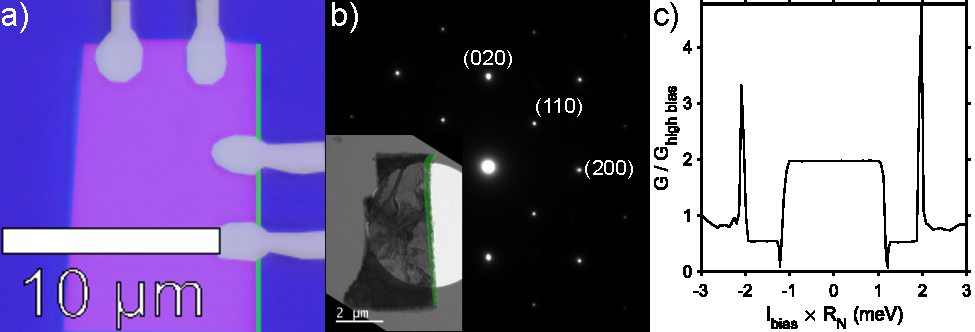
\includegraphics[width = \textwidth]{Chap4/Figures/DeviceFab.pdf}
	\caption{a) False color optical image of a representative device with a straight (100) edge highlighted in green. b) \ac{TEM} diffraction pattern demonstrating the (100) edge. Inset shows the flake measured as well as the diffraction aperture. c) Base temperature differential conductance curve.}
	\label{fig:PARDeviceFab}
\end{figure}
The tunneling conductance of a normal-metal/superconductor interface can be modeled by assuming an delta-function potential barrier at the interface characterized by a strength parameter $Z$, i.e., the \ac{BTK} method. An in-depth discussion and pseudo code for performing these simulations can be found in \ref{app:ARfit}], however we will take some of the main results of these calculations for discussions here. The \ac{BTK} method on a standard \ac{BCS} s-wave superconductor predicts a bias-independent conductance plateau only when the strength of the potential barrier between the normal-metal and superconductor is exactly zero. Even slight deviations from a zero-strength barrier result in significant dips around zero-bias, thus observing \ac{PAR} is exceedingly rare and typically only occurs only in extremely clean materials \cite{Lee2019}. Therefore when \ac{PAR} is observed in a system it is usually due to an underlying mechanism which causes the incoming carriers to ignore the barrier completely; these mechanisms include forbidden backscattering due to topological spin-momentum locked bands and majorana zero-mode assisted tunneling, among others. \ac{PAR} has three unique identifiers in a differential conductance spectrum: a perfectly flat plateau, the plateau is at twice the conductance of the normal state, and the plateau extends out to the superconducting energy gap.\par
\begin{figure}
	\centering
	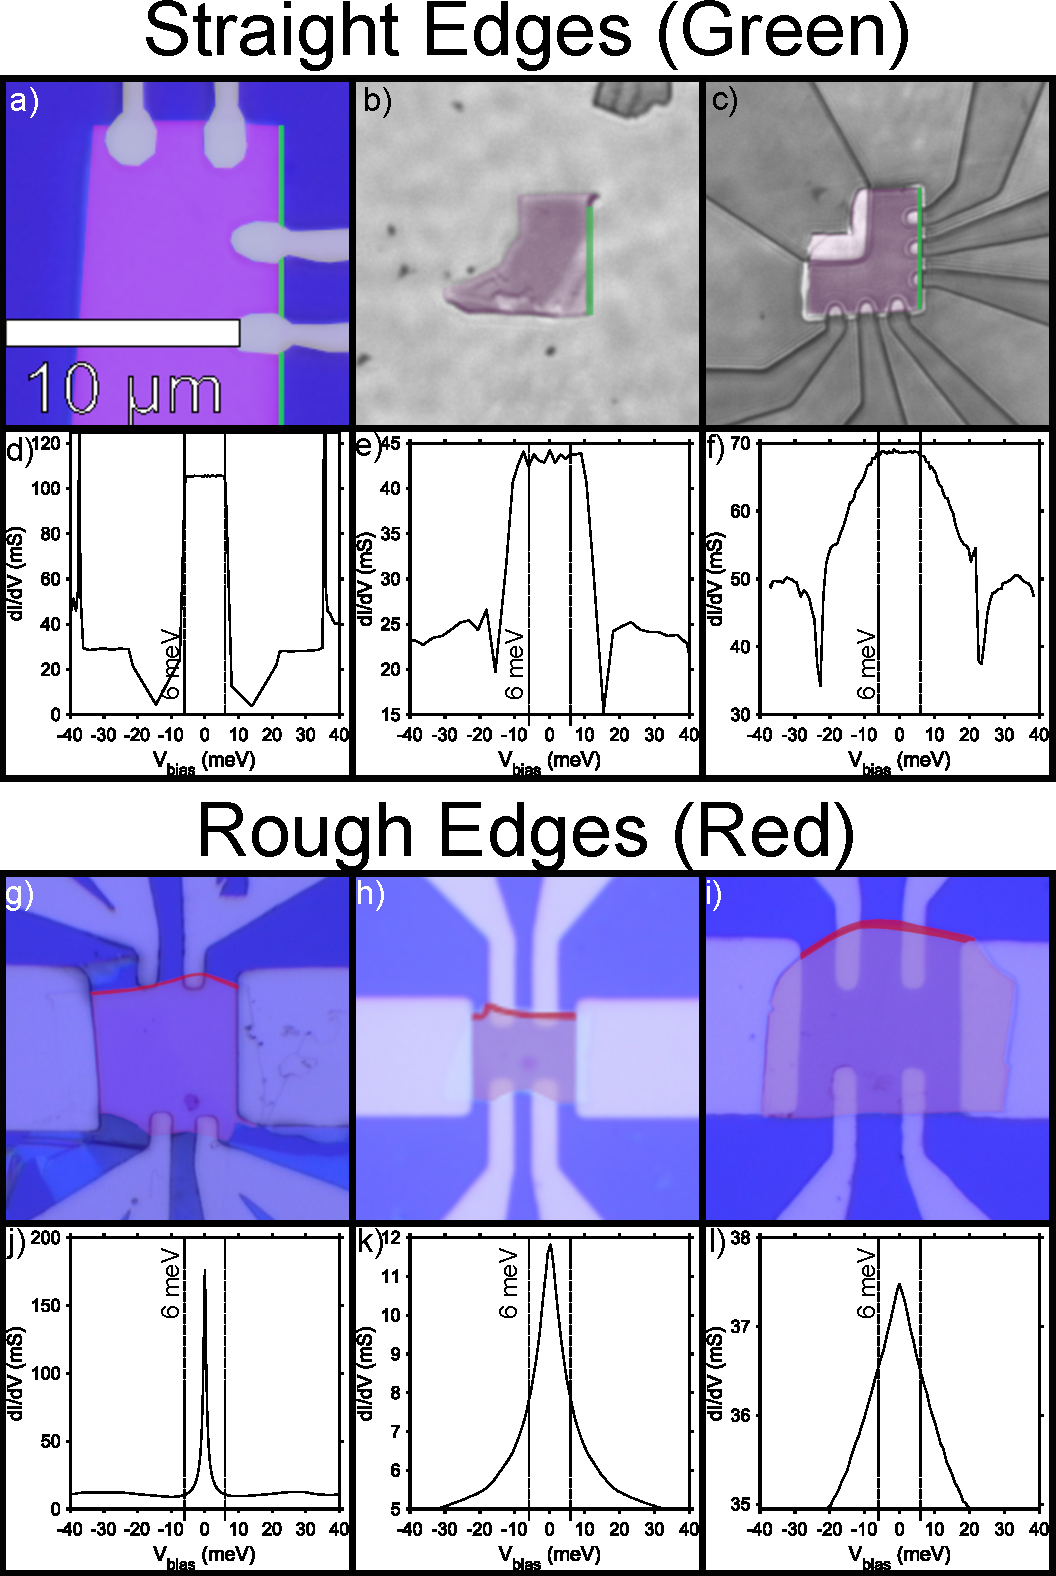
\includegraphics[scale = 0.75]{Chap4/Figures/StraightVsRough.pdf}
	\caption{Optical photos and associated conductance measurements of straight edges (a-f) versus rough edges (g-l). Measured edges are highlighted in either green or red. The dashed lines in the conductance graphs denote $\pm$6 meV.}
	\label{fig:StraightVsNormal}
\end{figure}
\begin{figure}
	\centering
	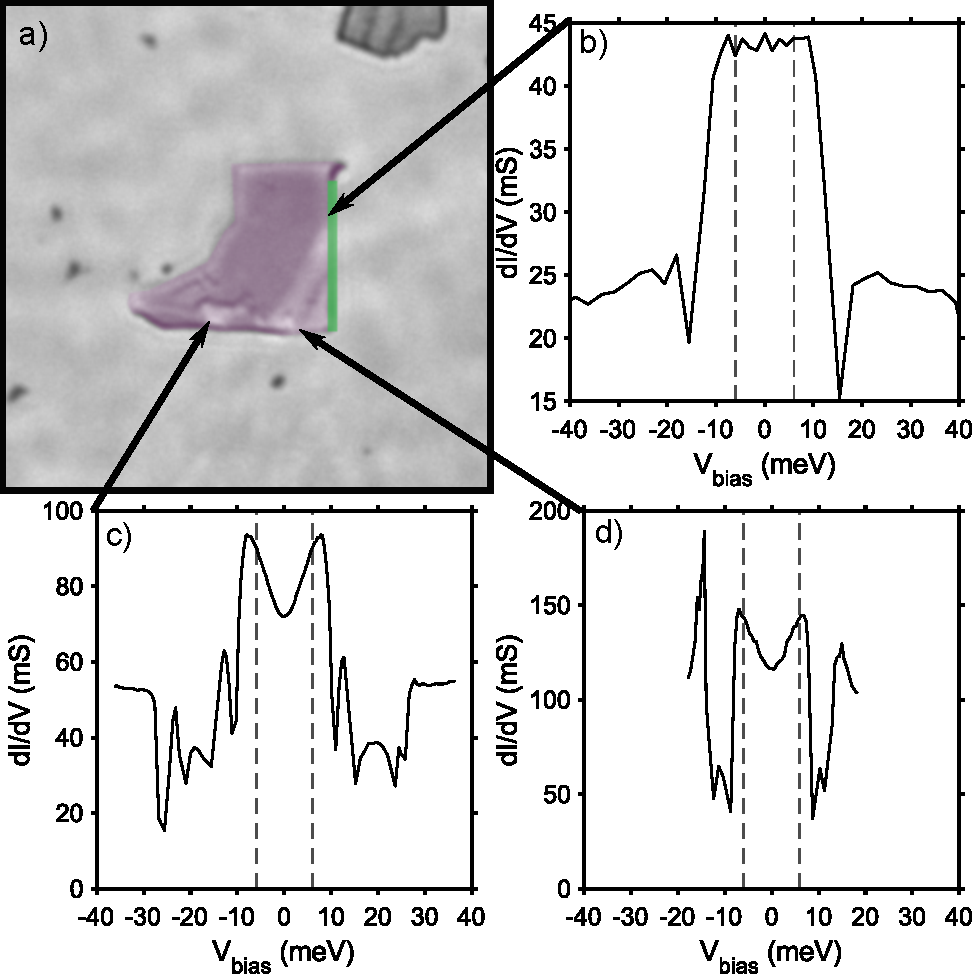
\includegraphics[width=\textwidth]{Chap4/Figures/ControlFlake.pdf}
	\caption{Measuring straight versus rough edges on the same device. a,b) Same data as seen in Fig \ref{fig:StraightVsNormal}. c,d) Differential conductance measured across the rough edge of the device in two different points.}
	\label{fig:ControlDevice}
\end{figure}
This bias-independent conductance plateau is observed in other devices with straight edges, however when performing tunneling experiments on ``rough" edges (i.e. edges that are not straight) the differential conductance does not show a plateau at low-biases (Fig \ref{fig:StraightVsNormal}). This suggests that either the \ac{PAR} in this system is sensitive to the local contact conditions or the contact to the bulk superconductivity is greatly increased with rough contacts. In the first case, the topological nature of \ac{FTS} would be immediately called into question as the topology should not be affected by local crystal symmetry breaking. Indeed, this would seem to indicate that \ac{FTS} would be something closer to a Topological Crystalline Insulator. In the latter case, the \ac{PAR} is not affected by the local contact conditions but the signal is drowned out among a much larger supercurrent when better contact is made to the superconducting bulk.\par
\begin{figure}[h]
    \centering
    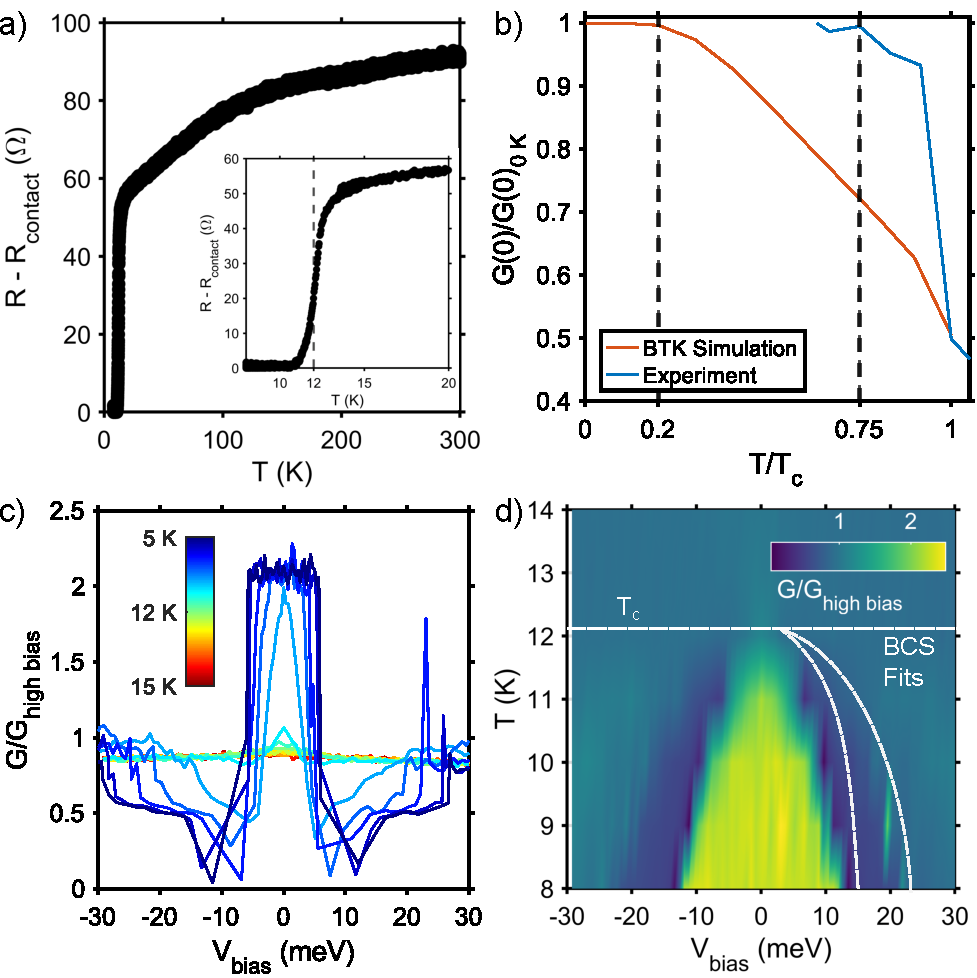
\includegraphics[width = \textwidth]{Chap4/Figures/Temperature.pdf}
    \caption{a) Two-point resistance with contact resistance subtracted out. b) Comparison of zero-bias conductance for the standard s-wave BTK simulation and our \ac{PAR} data. c) Differential conductance as a function of temperature. d) Colormap of differential conductance versus a current bias and temperature.}
    \label{fig:PARTemp}
\end{figure}
While the temperature dependence of the width of this \ac{PAR} follows the \ac{BCS} model quite well, there is a striking difference when comparing the conductance at zero-bias to the \ac{BTK} model. Indeed, while a \ac{BTK} calculation with $Z=0$ displays a zero-bias conductance saturating around $T=0.2T_{c}$ the measured zero-bias conductance in \ac{FTS} saturates at a far higher temperature around $T = 0.75T_{c}$. This provides further evidence that the \ac{PAR} is not simply caused by lucky, perfect contacts as it seems the mechanism is only limited by the magnitude of the superconducting gap not by temperature.  

\section{Magnetic Field Dependence}
The Dirac surfaces states that are a key signature of a topological bulk are protected via time-reversal symmetry. It follows that if time-reversal symmetry is lifted via a magnetic field, any Dirac nodes that are aligned (the plane perpendicular to the spin-momentum locking determines the ``direction" of the cone) along the magnetic field will lose their topological protection. In contrast, if the Dirac node is perpendicular to the magnetic field, the node will simply shift up or down in energy but the node will keep its topological protection. In this manner, if the \ac{PAR} is caused by forbidden backscattering due to topological bands we expect highly anisotropic responses to different directions of applied magnetic field. While this seems to be the case in \ac{FTS} (shown in Fig \ref{fig:PARField}) we must be careful to differentiate the response of the \ac{PAR} from that of the bulk superconductor. Even though the upper critical field of \ac{FTS} is around $35 T$\cite{Mele2012} the bulk superconducting response of \ac{FTS} flakes is quite anisotropic, even below $9 T$ \cite{zalic2019}. When applying a magnetic field parallel with the hinge being measured (the a-axis of the material), the \ac{PAR} remains completely unaffected up to $5 T$. However, when the field is rotated to the c-axis of the crystal the \ac{PAR} seems to collapse quite rapidly which would give credence to a topological origin as discussed earlier. 
\begin{figure}[h]
    \centering
    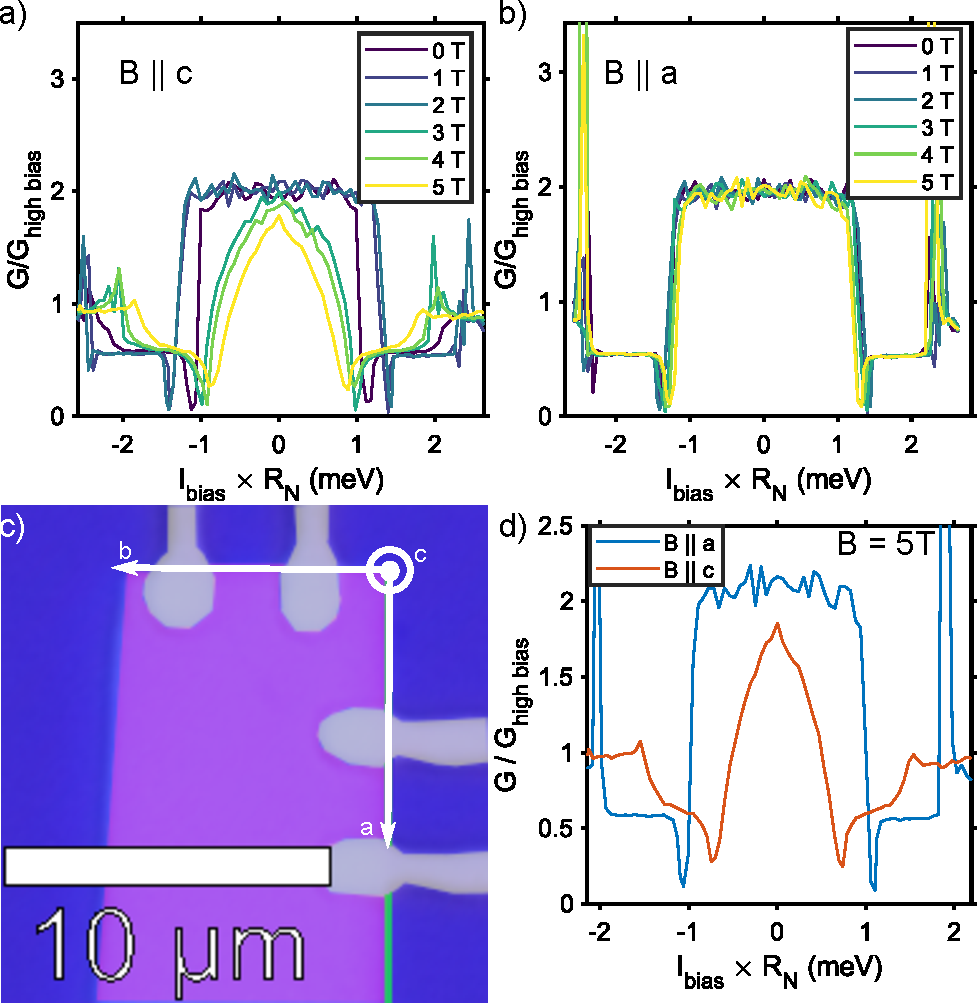
\includegraphics[width = \textwidth]{Chap4/Figures/MagneticField.pdf}
    \caption{Differential conductance as a function of magnetic field for a) a magnetic field that is parallel to the edge being measured and b) a magnetic field that is perpendicular to the magnetic field being measured. d) Comparison of conductance spectra at 5T for both magnetic field cases.}
    \label{fig:PARField}
\end{figure}
\section{Conclusion}
In this work we expanded upon the methods used in Chapter \ref{chap:CRAIG}. When contacting straight, crystallographic edges we observe \acl{PAR} while contacts on ``rough" edges displayed normal \acl{AR} spectra. 